% chapters/06-risk-management.tex

\chapter{Risk Management and Compliance}\label{ch:risk-management-and-compliance}

\begin{importantbox}
This chapter provides a comprehensive framework for identifying, assessing, and mitigating risks in the Nigerian market, along with detailed compliance requirements by sector and region.
\end{importantbox}

\section{Due Diligence Framework}\label{sec:due-diligence-framework}

\subsection{Core Due Diligence Components}\label{subsec:core-due-diligence-components}

\begin{figure}[htbp]
    \centering
    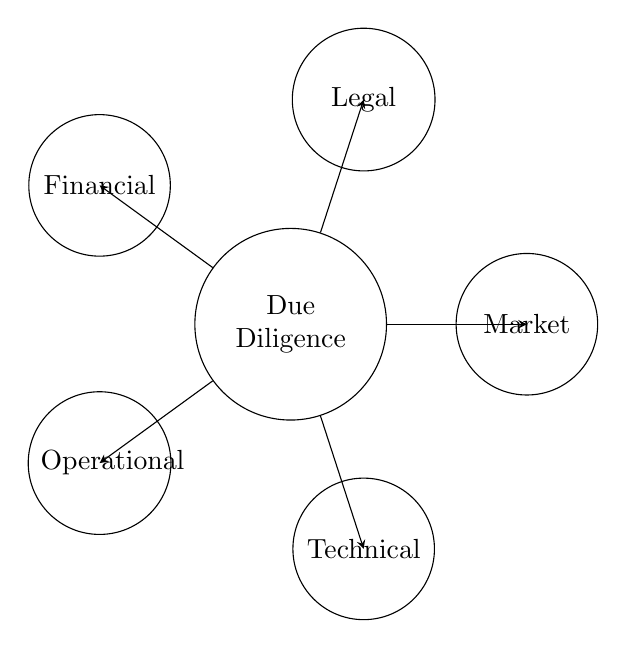
\begin{tikzpicture}[node distance=2cm]
        % Core node
        \node[draw, circle, text width=2cm, align=center] (core) {Due\\Diligence};

        % Surrounding nodes with better spacing
        \foreach \angle/\label in {
            0/Market,
            72/Legal,
            144/Financial,
            216/Operational,
            288/Technical
        } {
            \node[draw, circle, text width=1.5cm, align=center]
                at (\angle:3) {\label};
            \draw[-stealth] (core) -- (\angle:3);
        }
    \end{tikzpicture}
    \caption{Due Diligence Framework}
    \label{fig:due-diligence}
\end{figure}

\subsection{Risk Assessment Matrix}
\begin{center}
\begin{tabularx}{\textwidth}{>{\raggedright\arraybackslash}X >{\centering\arraybackslash}X >{\centering\arraybackslash}X >{\raggedright\arraybackslash}X}
    \toprule
    \textbf{Risk Type} & \textbf{Likelihood} & \textbf{Impact} & \textbf{Mitigation Strategy} \\
    \midrule
    Regulatory & High & High & Compliance partners \\
    Market & Medium & High & Phased entry \\
    Operational & Medium & Medium & Local expertise \\
    Financial & Medium & High & Risk management \\
    Technical & Low & Medium & Testing protocols \\
    \bottomrule
\end{tabularx}
\end{center}

\FloatBarrier
\section{Legal Safeguards}\label{sec:legal-safeguards}

\begin{warningbox}
Legal requirements can change frequently.\ Always verify current requirements through official channels or your legal counsel.
\end{warningbox}

\subsection{Essential Legal Documentation}\label{subsec:essential-legal-documentation}
\begin{tcolorbox}[colback=white,colframe=primarydark,title=\textbf{Documentation Checklist}]
\begin{itemize}
    \item Registration certificates
    \item Operating licenses
    \item Tax registrations
    \item Regulatory permits
    \item Employment contracts
    \item Partnership agreements
\end{itemize}
\end{tcolorbox}

\FloatBarrier
\section{Regional Compliance Requirements}\label{sec:regional-compliance-requirements}

\begin{regionalbox}{United Kingdom}
\textbf{Financial Services Compliance Framework}
\begin{itemize}
    \item \textbf{Central Bank of Nigeria (CBN) Requirements}
    \begin{itemize}
        \item Minimum capital requirement: NGN 25 billion for commercial banking
        \item Risk-based capital adequacy ratio: 15\%
        \item Non-performing loans ratio: maximum 5\%
        \item Liquidity ratio: minimum 30\%
        \item Daily reporting requirements for specified transactions
        \item Monthly returns submission
        \item Annual external audit
    \end{itemize}

    \item \textbf{Financial Conduct Authority (FCA) Requirements}
    \begin{itemize}
        \item Authorization application process
        \item Threshold Conditions compliance
        \item Systems and controls framework
        \item Senior Managers and Certification Regime
        \item Conduct risk management
        \item Client money protection
        \item Regular reporting obligations
    \end{itemize}

    \item \textbf{Anti-Money Laundering Regulations}
    \begin{itemize}
        \item Customer Due Diligence (CDD)
        \item Enhanced Due Diligence (EDD)
        \item Transaction monitoring systems
        \item Suspicious Activity Reporting (SAR)
        \item Record keeping requirements
        \item Staff training programs
        \item Regular risk assessments
    \end{itemize}

    \item \textbf{Data Protection Standards}
    \begin{itemize}
        \item Nigeria Data Protection Regulation compliance
        \item GDPR compliance for EU data
        \item Privacy impact assessments
        \item Data breach notification procedures
        \item Data retention policies
        \item Cross-border data transfer protocols
    \end{itemize}
\end{itemize}
\end{regionalbox}

\FloatBarrier
\subsection{UK Compliance Timeline}
\begin{figure}[htbp]
    \centering
    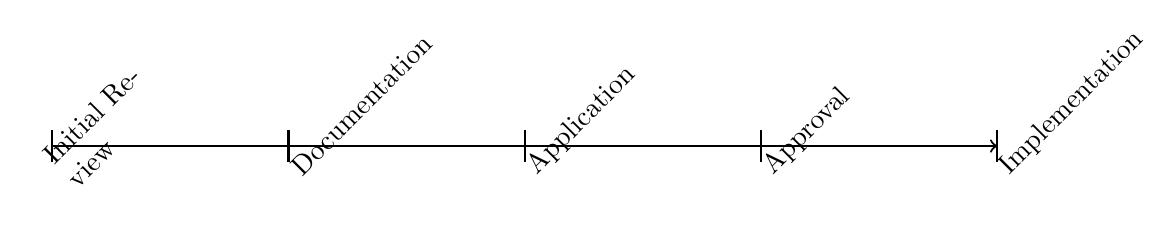
\begin{tikzpicture}
        % Timeline with better spacing and labels
        \draw[thick,->] (0,0) -- (12,0);
        \foreach \x/\label in {
            0/Initial Review,
            3/Documentation,
            6/Application,
            9/Approval,
            12/Implementation
        } {
            \draw[thick] (\x,0.2) -- (\x,-0.2);
            \node[text width=2cm, align=left, rotate=45, anchor=west]
                at (\x,-0.4) {\label};
        }
    \end{tikzpicture}
    \caption{UK Financial Services Compliance Process}
    \label{fig:uk-compliance}
\end{figure}

\begin{regionalbox}{United States}
\textbf{Tech Regulation and Data Protection}
\begin{itemize}
    \item \textbf{Data Privacy Requirements}
    \begin{itemize}
        \item NDPR compliance framework
        \item Privacy policy implementation
        \item Data collection consent
        \item Access rights management
        \item Breach notification protocols
        \item Regular privacy audits
    \end{itemize}

    \item \textbf{IP Protection Framework}
    \begin{itemize}
        \item Patent registration process
        \item Trademark protection
        \item Copyright registration
        \item Trade secret protocols
        \item Licensing agreements
        \item IP enforcement strategies
    \end{itemize}

    \item \textbf{Digital Security Compliance}
    \begin{itemize}
        \item Security assessment framework
        \item Penetration testing requirements
        \item Encryption standards
        \item Access control protocols
        \item Incident response planning
        \item Regular security audits
    \end{itemize}
\end{itemize}

\subsection{US Tech Compliance Matrix}\label{subsec:us-tech-compliance-matrix}
\begin{center}
\begin{tabularx}{\textwidth}{>{\raggedright\arraybackslash}X >{\centering\arraybackslash}X >{\raggedright\arraybackslash}X}
    \toprule
    \textbf{Requirement} & \textbf{Standard} & \textbf{Implementation} \\
    \midrule
    Data Privacy & NDPR/GDPR-aligned & Privacy framework \\
    Security & ISO 27001 & Security protocols \\
    Consumer Protection & FTC standards & Protection measures \\
    \bottomrule
\end{tabularx}
\end{center}
\end{regionalbox}

\begin{regionalbox}{UAE}
\textbf{Trade Compliance Framework}
\begin{itemize}
    \item \textbf{Trade License Requirements}
    \begin{itemize}
        \item General trading license
        \item Specific product licenses
        \item Agent registration
        \item Annual renewals
        \item Activity restrictions
    \end{itemize}

    \item \textbf{Import/Export Regulations}
    \begin{itemize}
        \item Documentation requirements
        \item Customs procedures
        \item Duty calculations
        \item Restricted items
        \item Special permissions
    \end{itemize}

    \item \textbf{Currency Controls}
    \begin{itemize}
        \item Transaction reporting
        \item Exchange controls
        \item Documentation requirements
        \item Transfer limits
        \item Compliance reporting
    \end{itemize}
\end{itemize}

\subsection{UAE Trade Compliance Checklist}\label{subsec:uae-trade-compliance-checklist}
\begin{tcolorbox}[colback=white,colframe=primary,title=\textbf{Required Documents}]
\begin{itemize}
    \item Trade license
    \item Chamber of Commerce registration
    \item Import/export permits
    \item Customs registration
    \item Bank references
\end{itemize}
\end{tcolorbox}
\end{regionalbox}

\begin{regionalbox}{Canada}
\textbf{Environmental and Agricultural Compliance}
\begin{itemize}
    \item Environmental standards
    \item Agricultural regulations
    \item Food safety requirements
    \item Export compliance
\end{itemize}

\subsection{Canadian Sector Compliance}\label{subsec:canadian-sector-compliance}
\begin{center}
\begin{tabularx}{\textwidth}{>{\raggedright\arraybackslash}X >{\centering\arraybackslash}X >{\raggedright\arraybackslash}X}
    \toprule
    \textbf{Sector} & \textbf{Standards} & \textbf{Certifications} \\
    \midrule
    Agriculture & CFIA standards & Safety certificates \\
    Environment & ISO 14001 & Environmental permits \\
    Food Processing & HACCP & Safety certifications \\
    \bottomrule
\end{tabularx}
\end{center}
\end{regionalbox}

\FloatBarrier
\section{Banking and Money Transfer}\label{sec:banking-and-money-transfer}

\subsection{Banking Structure}\label{subsec:banking-structure}
\begin{figure}[htbp]
    \centering
    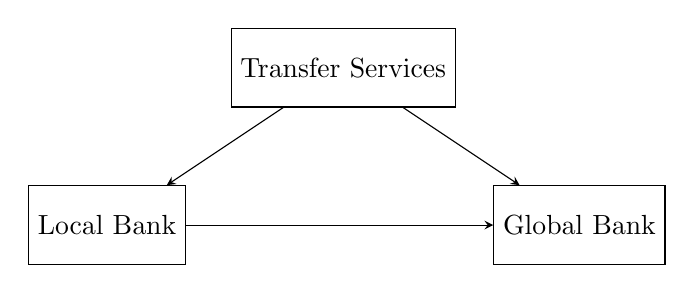
\begin{tikzpicture}[
        node distance=2cm,
        box/.style={draw, minimum width=2cm, minimum height=1cm}
    ]
        % Banking structure diagram with improved spacing
        \node[box] (local) at (0,0) {Local Bank};
        \node[box] (global) at (6,0) {Global Bank};
        \node[box] (transfer) at (3,2) {Transfer Services};
        \draw[-stealth] (local) -- (global);
        \draw[-stealth] (transfer) -- (local);
        \draw[-stealth] (transfer) -- (global);
    \end{tikzpicture}
    \caption{Cross-Border Banking Structure}
    \label{fig:banking-structure}
\end{figure}

\subsection{Banking Operations Framework}\label{subsec:banking-operations-framework}
\begin{tcolorbox}[colback=white,colframe=primarydark,title=\textbf{Banking Operations Components}]
\begin{itemize}
    \item \textbf{Account Setup}
    \begin{itemize}
        \item Corporate account requirements
        \item Documentation process
        \item Signatory arrangements
        \item Online banking setup
        \item Mobile banking activation
    \end{itemize}

    \item \textbf{Transaction Processing}
    \begin{itemize}
        \item Payment authorizations
        \item Transaction limits
        \item Processing timeframes
        \item Fee structures
        \item Reconciliation procedures
    \end{itemize}

    \item \textbf{Cross-Border Operations}
    \begin{itemize}
        \item International transfer protocols
        \item Documentation requirements
        \item Correspondent banking relationships
        \item Compliance procedures
        \item Reporting obligations
    \end{itemize}
\end{itemize}
\end{tcolorbox}

\FloatBarrier
\section{Currency Risk Management}\label{sec:currency-risk-management}

\subsection{Hedging Strategies Framework}\label{subsec:hedging-strategies-framework}
\begin{tcolorbox}[colback=white,colframe=primarydark,title=\textbf{Currency Risk Mitigation Strategies}]
\begin{itemize}
    \item \textbf{Forward Contracts}
    \begin{itemize}
        \item Contract specifications
        \item Pricing mechanisms
        \item Settlement procedures
        \item Documentation requirements
        \item Risk assessment
    \end{itemize}

    \item \textbf{Currency Hedging}
    \begin{itemize}
        \item Options strategies
        \item Swap arrangements
        \item Natural hedging
        \item Cross-currency hedging
        \item Cost considerations
    \end{itemize}

    \item \textbf{Local Currency Management}
    \begin{itemize}
        \item Account structuring
        \item Conversion timing
        \item Balance optimization
        \item Interest management
        \item Exposure limits
    \end{itemize}
\end{itemize}
\end{tcolorbox}

\begin{communitybox}
Access additional risk management resources on the Africa Growth Circle:
\begin{itemize}
    \item Risk assessment templates
    \item Compliance checklists
    \item Expert advisory sessions
    \item Regulatory updates
    \item Due diligence guides
\end{itemize}
Visit circle.counseal.com for risk management support.
\end{communitybox}

% End of chapter workshop
\begin{workshopbox}
\textbf{Chapter 6 Risk Management Workshop}

1. Risk Assessment
\begin{itemize}
    \item Key risks identified: \_\_\_\_\_\_\_\_\_
    \item Risk priority ranking: \_\_\_\_\_\_\_\_\_
    \item Mitigation strategies: \_\_\_\_\_\_\_\_\_
\end{itemize}

2. Compliance Planning
\begin{itemize}
    \item Required permits: \_\_\_\_\_\_\_\_\_
    \item Documentation needed: \_\_\_\_\_\_\_\_\_
    \item Timeline for completion: \_\_\_\_\_\_\_\_\_
\end{itemize}

3. Banking Structure
\begin{itemize}
    \item Banking partners: \_\_\_\_\_\_\_\_\_
    \item Transfer mechanisms: \_\_\_\_\_\_\_\_\_
    \item Currency management: \_\_\_\_\_\_\_\_\_
\end{itemize}

Download comprehensive risk assessment templates from the Africa Growth Circle platform.
\end{workshopbox}

\begin{importantbox}
In Chapter 7, we'll explore building your local network and establishing key partnerships to help manage risks and ensure compliance.
\end{importantbox}